\chapter{Eletrônica Embarcada}

\subsubsection{Conversor Analógico/Digital}

\begin{enumerate}
  \item Conversor Analógico/Digital
  \begin{enumerate}
    \item Definição

    Os sinais que existem no mundo real são analógicos e, por essa razão, esses sinais devem ser transformados em digitais por meio de um conversor, para que possam ser manipulados pelo equipamento digital.

    Um conversor analógico/digital, também conhecido com A/D ou ADC, é um dispositivo que gera um sinal digital a partir de um analógico. Normalmente, esse sinal analógico é o valor de uma tensão ou corrente. Esses instrumentos são utilizados na interface entre dispositivos digitais e analógicos. Uma das grandes vantagens de se obter um valor digital é a capacidade de compactação de dados, podendo diminuir o tamanho do arquivo, economizando espaço na largura de banda, que é uma dos limitadores do conversor. Geralmente, é utilizando um filtro passa-baixas antes do conversor A/D, com o objetivo de evitar que amplitudes de alta frequência apareçam na entrada do conversor.

    \item Funcionamento

    Os microcontroladores processam dados obtidos por sensores. No entanto, na saída dos sensores é encontrado valores analógicos, logo é necessário transformá-los em valores digitais. Então, para executar essa atividade, é preciso do conversor A/D, que interfaceiam os dispositivos de medidas, e o microcontrolador \ref{fig:conversorAD}

    \begin{figure}[h]
      \centering
      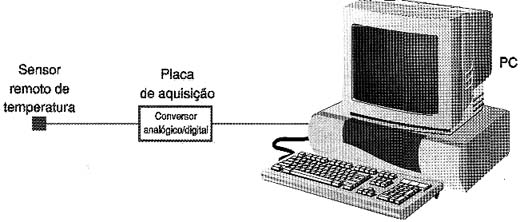
\includegraphics[width=0.25\textwidth]{figuras/conversorAD}
      \caption{Conversão A/D}
      \label{fig:conversorAD}
    \end{figure}

    \item Nanoshield ADC
  \end{enumerate}
\end{enumerate}
